% !TEX root = ../notes_template.tex
\chapter{Micro-circulatory support of Extracellular Fluid}\label{chp:ecf_microcirculation}
Updated on \today
\minitoc

%Capillary to ECF connection, transport of material, capillaries are a particular sieve ?spelling - how rapidly does circulation happen, pressure changes, lymph at the cellular level, why lymph? 

Muscle fibers are dependent on the extra cellular fluid (ECF) environment. The ECF is dependent on the micro-circulation. Water, ions, molecules and nutrients are constantly circulating between the vascular (capillaries and lymphatics) and interstitial compartments of the ECF. Exchange between the ECF and intra-cellular fluid (ICF) is more selective for ions, molecules and nutrients but comparatively free for water. The function of muscle fibers depends on the homeostasis of ECF oxygen, carbon dioxide, sodium, potassium, calcium, water, pH, and temperature.

\vspace{5mm}

\textbf{Objectives include:}
\begin{enumerate}
    \item Explain the basic dependency of muscle fibers on the extra-cellular fluid.
    \item Explain the basic dependency of extra-cellular fluid on the micro-circulation, circulation, renal filtration, respiration, ventilation, digestion, absorption, metabolism and elimination.
    \item
    \item
    \item
    \item
\end{enumerate}

\section{Part II: Muscle Support Overview}

The chapters of Part II are all about the supportive environment of the ECF. Every chapter describes a set of functions that serve the purpose of delivering, removing or regulating the contents of the ECF. This chapter focuses on the process of micro circulation of water and filtration of ions, molecules, nutrients and heat between the  vascular compartment of the ECF and the interstitial compartment, the non vascular compartment of the ECF.  

Figure \ref{fig:part2_overview} is a graphic representation of the chapters of Part II. Filtration relies on micro-circulation which relies on circulation. Circulation is the flow of blood through the entire circulatory system, covered in Chapter \ref{chp:blood_flow} on Blood Flow. Circulation of blood through the entire body ensures regular mixing of the ECF contents throughout the body. This mixing ensures consistency of ECF contents and a stable environment for all the cells of the body. For example, if blood $Na^+$ concentration is tested, it is properly assumed that concentration is the concentration of $Na^+$ throughout the entire ECF. Circulation also allows that each supporting system contribute - either to adding water, heat, ions, molecules or nutrients to the ECF, or removing by-products. Supporting systems are also in communication with one another based on the circulating substances and messages (hormones). For example, if a muscle working at high tension is shuttling lactate into the ECF, it is picked up by the circulation and can then enter other cells (heart, liver, non working muscles) where lactate levels are low. In these cells the lactate can be used to produce an $NADH$ from $NAD^+$, and a pyruvate to proceed into the mitochondria. The circulation is the nationwide transportation and distribution system that gets a package from the local post office to a post office across the country. The micro circulation is the delivery from the local post office to and from a mailbox at an address.

The contents of blood is regulated and supported by the renal (kidneys) and endocrine system, covered in Chapter \ref{chp:blood_content} on Blood Volume. The regular circulation of blood through the kidneys involves several mechanisms that regulate the ECF, and therefore the ICF, fluid volume. The regulation of fluid volume includes the regulation of several important ions (electrolytes) and the removal of waste (i.e. urea). Working with the endocrine system the kidneys provide long term regulation of blood pressure, which is important for circulation; as well as red blood cells, which is important for oxygen carrying capacity.

Cellular respiration in the mitochondria is constantly using the $O_2$ and producing $CO_2$. These molecules are called gases (blood, alveolar) because their natural state is in the gaseous form. The micro circulation ensures the regular delivery and removal of these gases from the interstitial fluid. The circulation to the lungs ensures the regular exchanges of these gases with the environment. Blood gases rely on blood flow through the lungs for respiration (gas exchange) between the blood and alveoli, covered in Chapter \ref{chp:blood_oxygen} on Blood Gas. Respiration depends on ventilation, the regular movement of these gases into and out of the lungs with the bulk transport of air. Ventilation is covered in \ref{chp:alveolar_oxygen} on Alveolar Gas. 

Maintaining blood nutrients relies on digestion, absorption, metabolism and elimination by the gastrointestinal organs and the liver. Based on the basic physiological concept of mass balance the regular elimination of water requires the regular intake of water. The regular transformation of the carbon bond energy from carbohydrates and fats requires the regular intake of carbohydrates and fat. The regular use, breakdown and elimination of proteins for cellular functions requires the regular intake of protein. All together these processes are covered in Chapter \ref{chp:blood_nutrients} on Visceral Support.

\begin{figure}[!h]
    \centering
    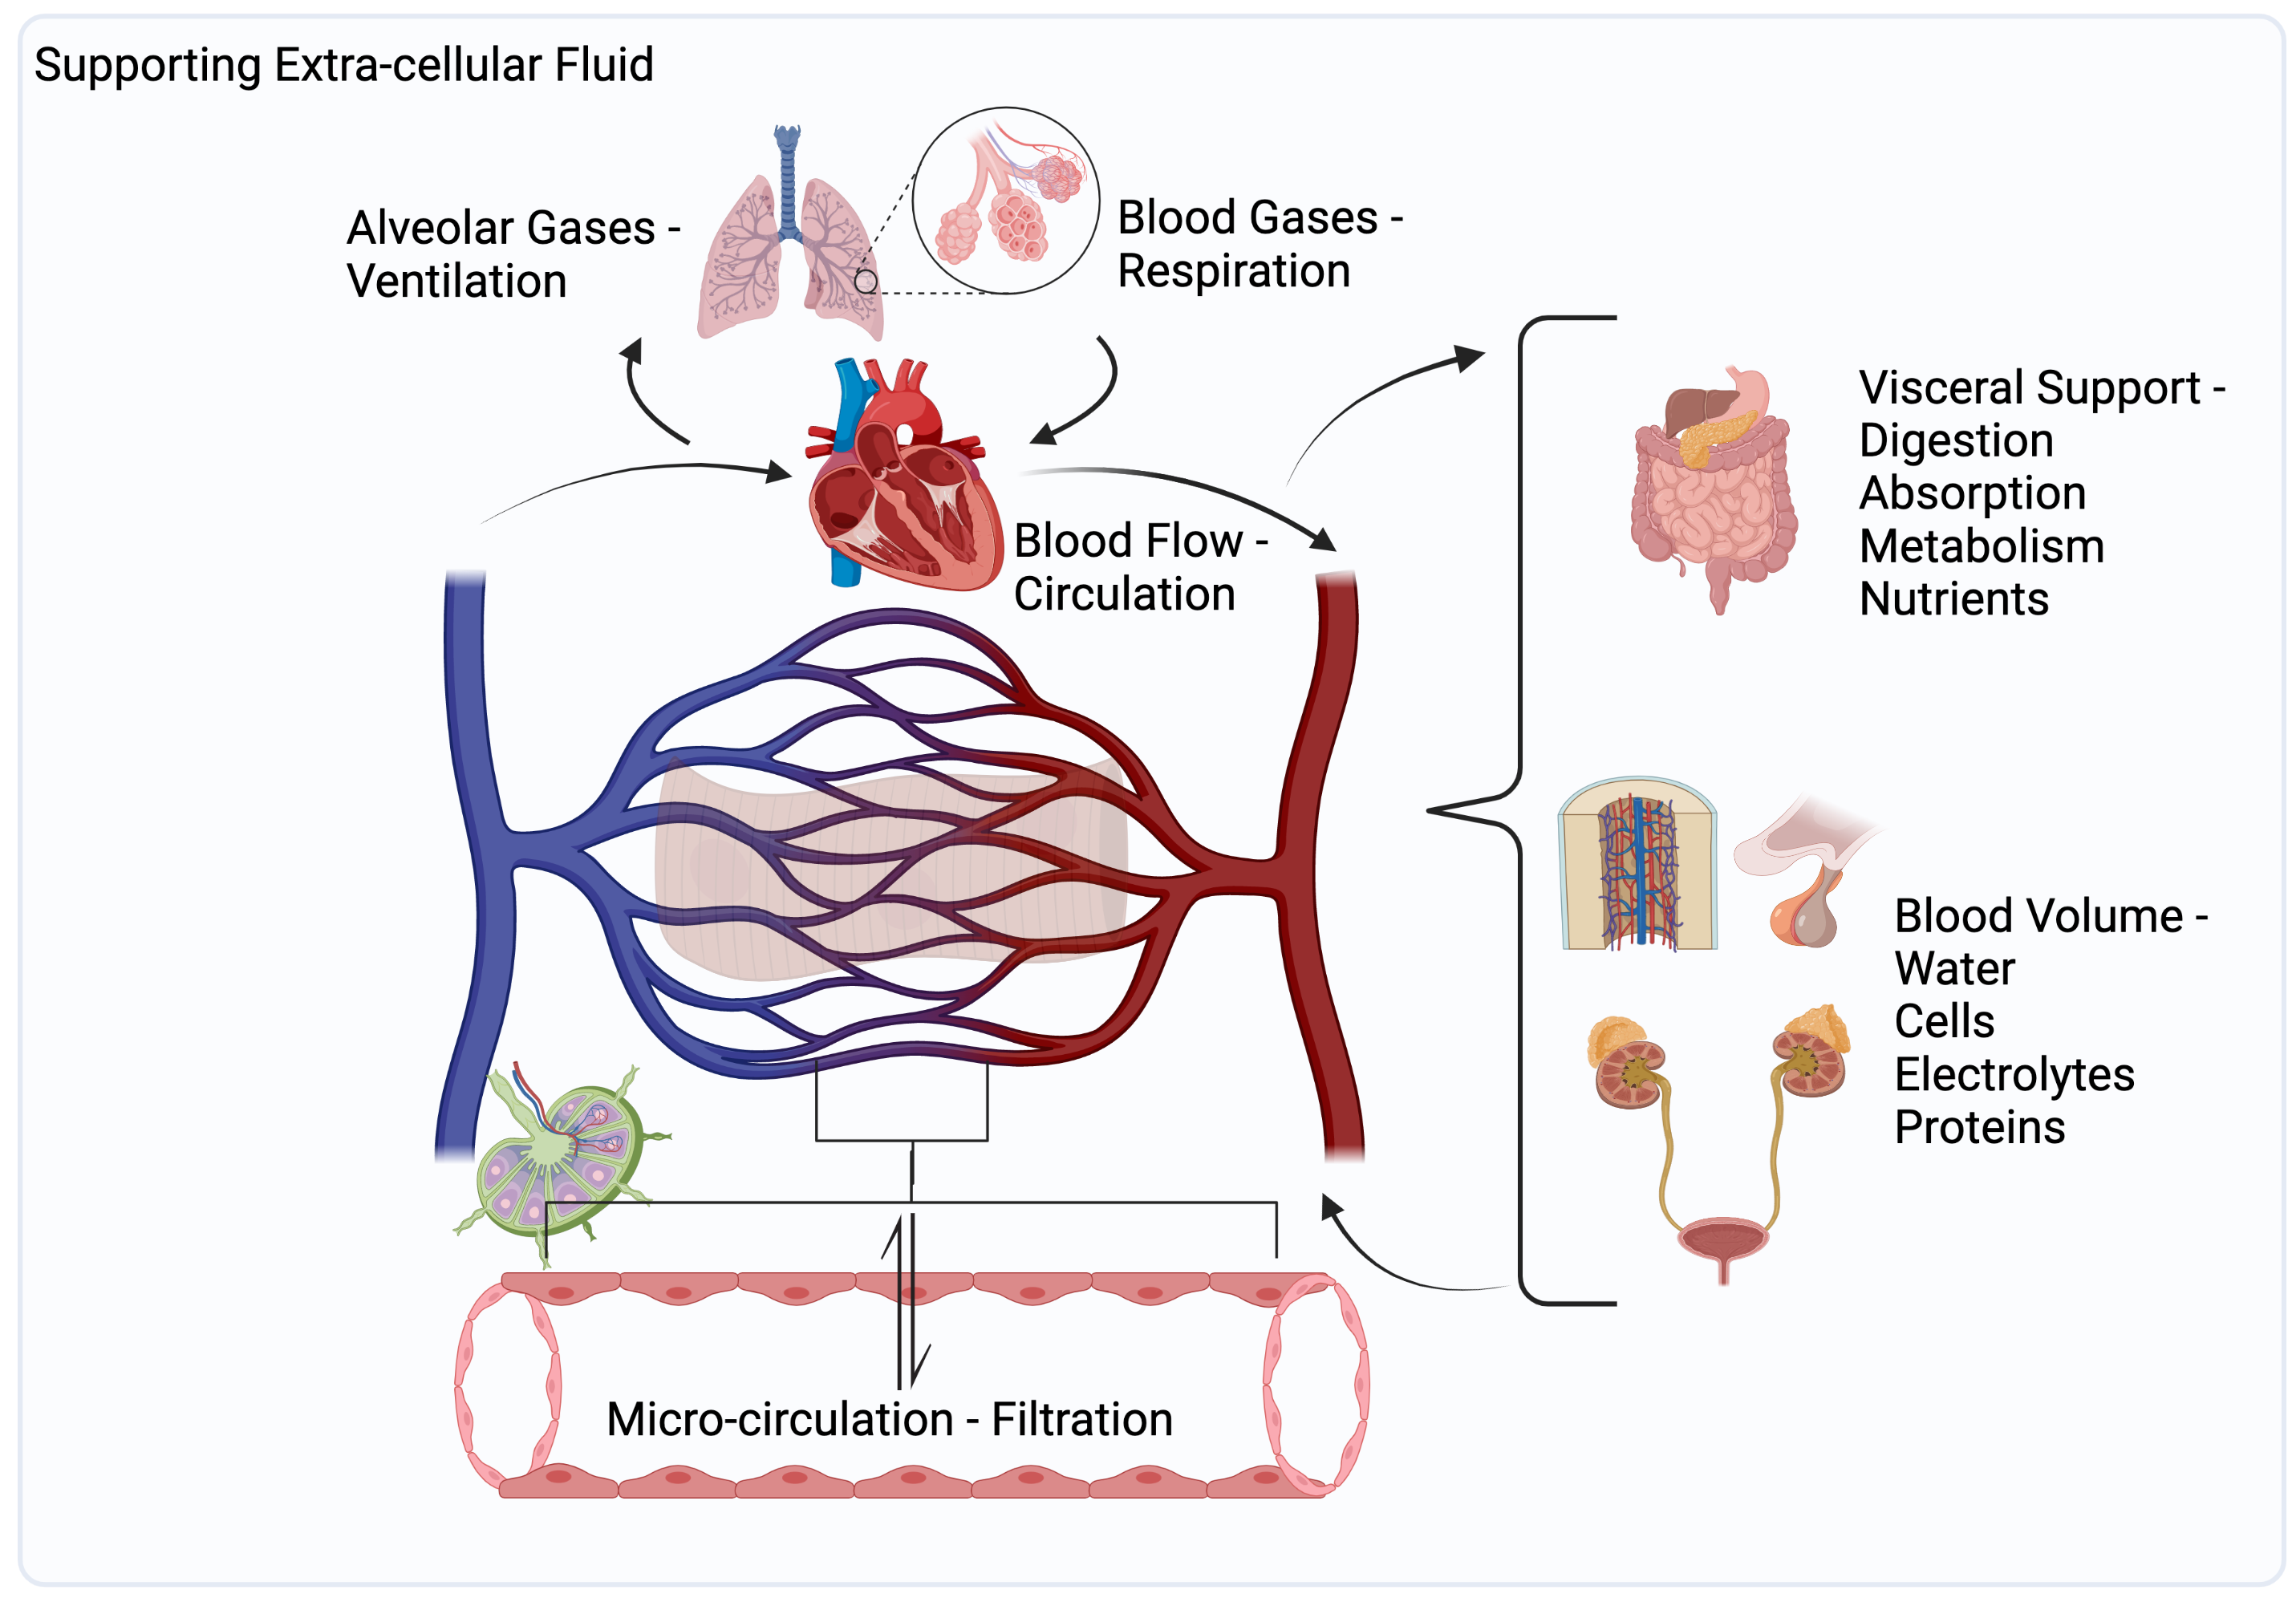
\includegraphics[width=1\linewidth]{./figure/part2_overview.png}
    \caption{Part II: Muscle Support Overview \footnotesize{Created with BioRender.com}}
    \label{fig:part2_overview}
\end{figure}

Together these systems support the ECF and therefore muscle fibers and muscle function. They maintain homeostasis of several important electrolytes (ions, including $H^+$ as measured by pH), nutrients, molecules, water and heat (temperature). They are integrated with several interactions and redundancies to provide support across a wide range of muscle demands in a wide range of circumstances, both good and bad.

\section{Micro Circulation}

Between 50-70\% of an adult body is fluid. The variation in the percent of the adult body that is fluid is based on variations in lean (mostly muscle) tissue. In individuals with more muscle (particularly compared to adipose tissue) there is a higher percent of water. Of the total body fluid approximately 2/3 is intracellular (ICF) and 1/3 is extra cellular (ECF). The ECF includes two compartments. The vascular compartment includes the circulating blood, and the interstitial (inside tissue, in between cells) compartment. The fluid component of the blood is plasma. 

Movement of ions, nutrients and molecules between the blood plasma and interstitial fluid occurs through the semi permeable capillary membranes in a process called filtration. The capillary membranes allow relatively free passage of water, ions, nutrients (other than proteins) and molecules. Other than protein content (particularly albumin), which is limited due to an inability of albumin to pass through the capillary membrane, and $O_2$ and $CO_2$ which is different due to constant exchange with the cell, the contents of vascular and interstitial fluid is similar. 

Exchange between the interstitial fluid and intracellular fluid occurs through the semi permeable cell membrane (muscle fiber cell membrane is the sarcolemma). The sarcolemma largely restricts movements of ions and even with changes in the permeability for $Na^+$ and $K^+$ during excitation does not change the concentration difference between the interstitial and ICF fluid for these ions (at least under normal circumstances). The sarcolemma regulates the movement of nutrients.  Glucose uptake by a cell is influenced by the activation of the glut4 receptor channel for glucose by insulin. Water moves freely between the interstitial and ICF due to a large quantity of aquaporins (water channels) in the membrane. The balance of ICF (2/3) and ECF fluid (1/3) water is therefore based largely on solute concentrations and resultant balance of osmotic pressure.

\subsection{Extra cellular \& Intra cellular Values \& Ranges}

Normal values of several important ions, nutrients and molecules are depicted in Figure \ref{fig:ecf}. Vascular and interstitial values are typically equal unless otherwise noted. $O_2$ and $CO_2$ pass easily through both the semipermeable capillary membrane and the semipermeable sarcolemma. Even at rest there is a relatively large gradient for these molecules. 

\begin{figure}[!h]
    \centering
    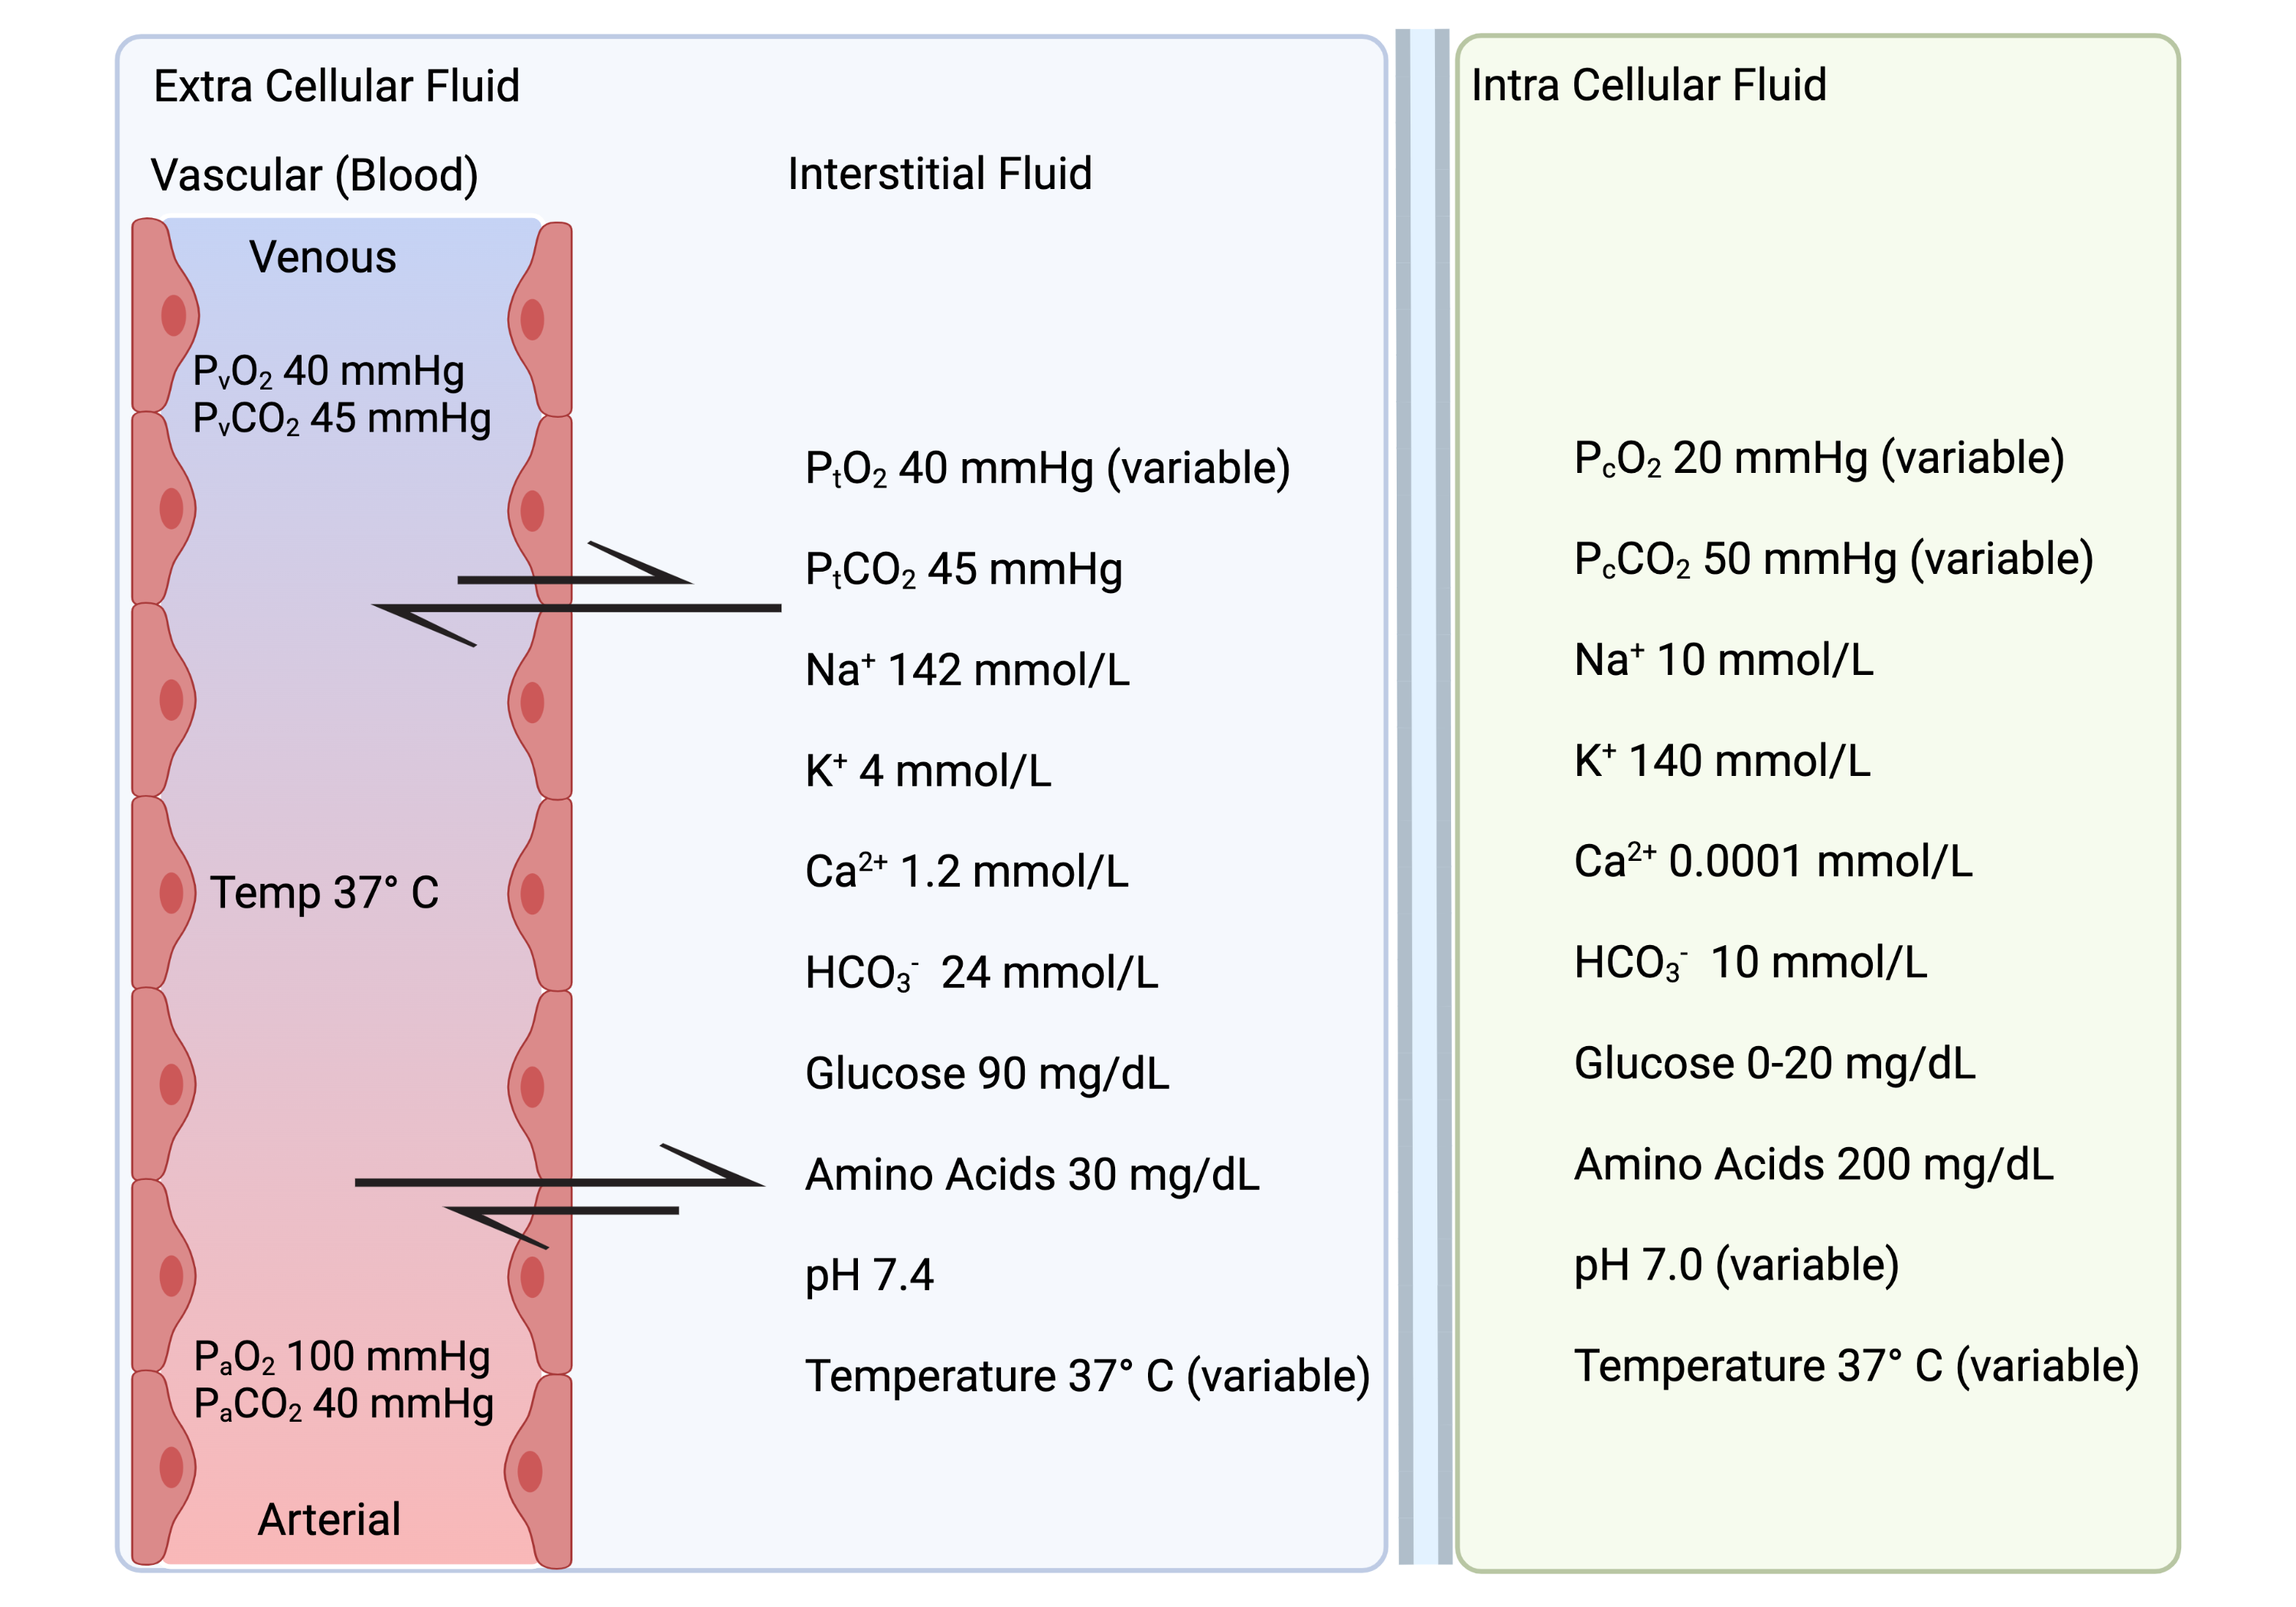
\includegraphics[width=1\linewidth]{./figure/ecf.png}
    \caption{Extra-cellular (Vascular \& Interstitial) and Intra-cellular Fluid \footnotesize{Created with BioRender.com}}
    \label{fig:ecf}
\end{figure}

Table \ref{table:ecf_value_ranges} provides normal values and ranges and non lethal limits for several important components of the extra cellular fluid.  The wide normal ranges and non lethal limit ranges is a good example of the degree of overall robustness in physiology systems. Moving outside of a range without an easy temporary explanation (such as low $P_v O_2$ in response to exercise) is an indication that something is wrong. But even when something is wrong, the body adjusts and even large deviations in normal values are tolerated before the changes become lethal. Several of these components of the ECF have larger non lethal limits in one direction. For example, $P_v O_2$ can increase tremendously (if given a large amount of oxygen in hyperbaric (high pressure) systems) before it becomes lethal. The criteria for lethal for these values is death. Some of the secondary effects may lead to premature death. For example, while a $Na^+$ value of 165 is within the non lethal limit, this value would be associated with, amongst other signs and symptoms of hypernatremia, a high blood volume and therefore high blood pressure despite attempts to maintain normal blood pressure. The elevated blood pressure can then lead to premature death.  Tolerance for temperature is greater with cold than with heat. With heat proteins denature and metabolic functions cannot be catalyzed. With decreased temperature reactions slow down from reduced kinetic energy, but at least the enzymes (proteins) are functioning. 

\begin{table}[h!]
\centering
\begin{tabular}{||c c c c||} 
 \hline
Value & Normal Value & Range & Non-Lethal Limit\\ [0.5ex] 
 \hline\hline
 $P_v O_2$ (mmHg) & 40  & 25-40 & 10-1000 \\
 $P_v CO_2$ (mmHg) & 45 & 41-51 & 5 - 80\\ 
 $Na^+$ (mmol/L) & 142 & 135 - 145 & 115 - 175\\
 $K^+$  (mmol/L) & 4.2 & 3.5 - 5.3 & 1.5 - 9.0\\ 
 $Ca^{2+}$ (mmol/L) & 1.2 & 1.0 - 1.4 & 0.5 - 2.0 \\
 $HCO_3 ^-$ (mmol/L)& 24 & 22 - 29 & 8 - 45 \\
 Glucose (mg/dL)& 90 & 70 - 115 & 20 - 1500 \\
 Acid-Base (pH) & 7.4 & 7.3 - 7.5 & 6.9 - 8.0 \\
 Temperature F (C) & 98.6 (37) & 98-98.8 (37) & 65-110 (18.3-43.3)[1ex] 
 \hline
\end{tabular}
\caption{Normal Range and Non Lethal Limits of Values in ECF (\footnotesize{Data from \cite{feher_quantitative_2017}})}
\label{table:ecf_value_ranges}
\end{table}

\subsection{Oxygen \& Carbon Dioxide}

The gradient for $O_2$ from the vascular fluid into the cell because the cell is constantly utilizing $O_2$. The gradient for $CO_2$ from the cell to the vascular fluid since the cell is constantly producing $CO_2$. The other gradient for $O_2$ and $CO_2$ depicted in Figure \ref{fig:ecf} is from the arterial end of the capillary to the venous end of the capillary. As shown, with healthy capillaries, normal capillary blood flow and normal blood the vascular $O_2$ and $CO_2$ partial pressure equilibrate by the time blood reaches the venous end of the capillary. The cellular and interstitial partial pressure for oxygen ($P_c O_2$ \& $P_t O_2$) are variable based on how much $O_2$ is being consumed in the muscle fiber, which is dependent on the rate of ATP regeneration occurring in electron transport (ETC). With a higher than resting ATP regeneration in ETC the $P_c O_2$ will drop, which drops the $P_t O_2$ below 40 mmHg, and then the partial pressure of oxygen at the venous end $P_v O_2$ of the capillary will also drop. $P_v O_2$ will equilibrate to $P_t O_2$. However, the $P_a O_2$ will remain at 100 mmHg as long as the circulation and pulmonary systems are providing the additional support that is required.

Similarly, for ETC to be regenerating ATP at a higher rate, TCA has to be functioning at a higher rate and thus producing more $CO_2$. This results in a higher $P_c CO_2$. However, because $P_t CO_2$ and $P_v CO_2$ equilibrate, as long as the circulation and pulmonary systems are providing the additional support that is required there will not be an increase in either $P_t CO_2$ or $P_v CO_2$.

\subsection{Temperature}

Temperature is heat unless there is a temperature of 0 degrees Kelvin. Heat is a byproduct of all energetic transformations, including regenerating ATP and hydrolyzing ATP. At rest temperature in muscle fiber equilibrates with that of the body because the flow of heat from the cells into the ECF is moved to the blood and out of the region. Some of the heat also dissipates through the ECF and tissues across the temperature gradient directly out of the body. When core body temperature falls, a reflex action is to shiver, which utilizes muscle activity to generate more heat for sharing with the rest of the body through the transport of ECF. When muscle temperature rises during activity, the circulation of blood carries much of that heat away from the muscle for dissipation throughout the body. As heat rises, more of the circulation is sent to the skin to facilitate this process.

\subsection{Water}

Cell membranes are permeable to water, but not to the ions. In steady state conditions the osmolarity between the ECF and ICF is approximately equal. Movement of fluid between the ICF and ECF is determined primarily by the osmosis. Changes in the concentration of solute (ions, molecules, nutrients) in the ECF and ICF changes the osmolarity and results in movement of water until osmolarity balance is achieved.

\subsubsection{Osmosis, Osmoles, Osmolarity \& Osmotic Pressure}

At this point most people need a review of these terms and the associated process of osmosis and osmotic pressure. 


Osmotic pressure is the pressure required to prevent osmosis of water through a semi permeable membrane that is permeable to water but not to the solute.

Osmoles (Osm) are the number of moles of solute that contribute to the osmotic pressure of a solution. The term comes from the phenomenon of osmosis, and is typically used for osmotically active solutions.

Osmolality is measuring the number of osmoles in a weight (kg) of solvent. Osmolarity is measure the number of osmoles in a volume (L) of solvent. Osmolarlity = Osm / Liter. Osmolarity is proportional to the milli osmoles / L as well (mOsm/L).

Osmotic pressure ($\pi$) is directly proportional to the concentration gradient of solutes ($C$), the ideal gas constant ($R$) and absolute temperature ($K = 310^{\circ}$ at body temperature): $\pi = C \cdot R \cdot T$. At body temperature each 1 mOSM/L (milli osmole per liter) difference in solute concentration results in approximately 19.3 mmHg of osmotic pressure. This means 19.3 mmHg of pressure is required to stop the movement of water if there is a 1 mOSM/L concentration gradient, or that 19.3 mmHg of pressure is generated by a difference of 1mOSM/L concentration gradient. Therefore, small differences in solute concentrations across a cell membrane results in rapid osmosis of water.

\begin{figure}[!h]
    \centering
    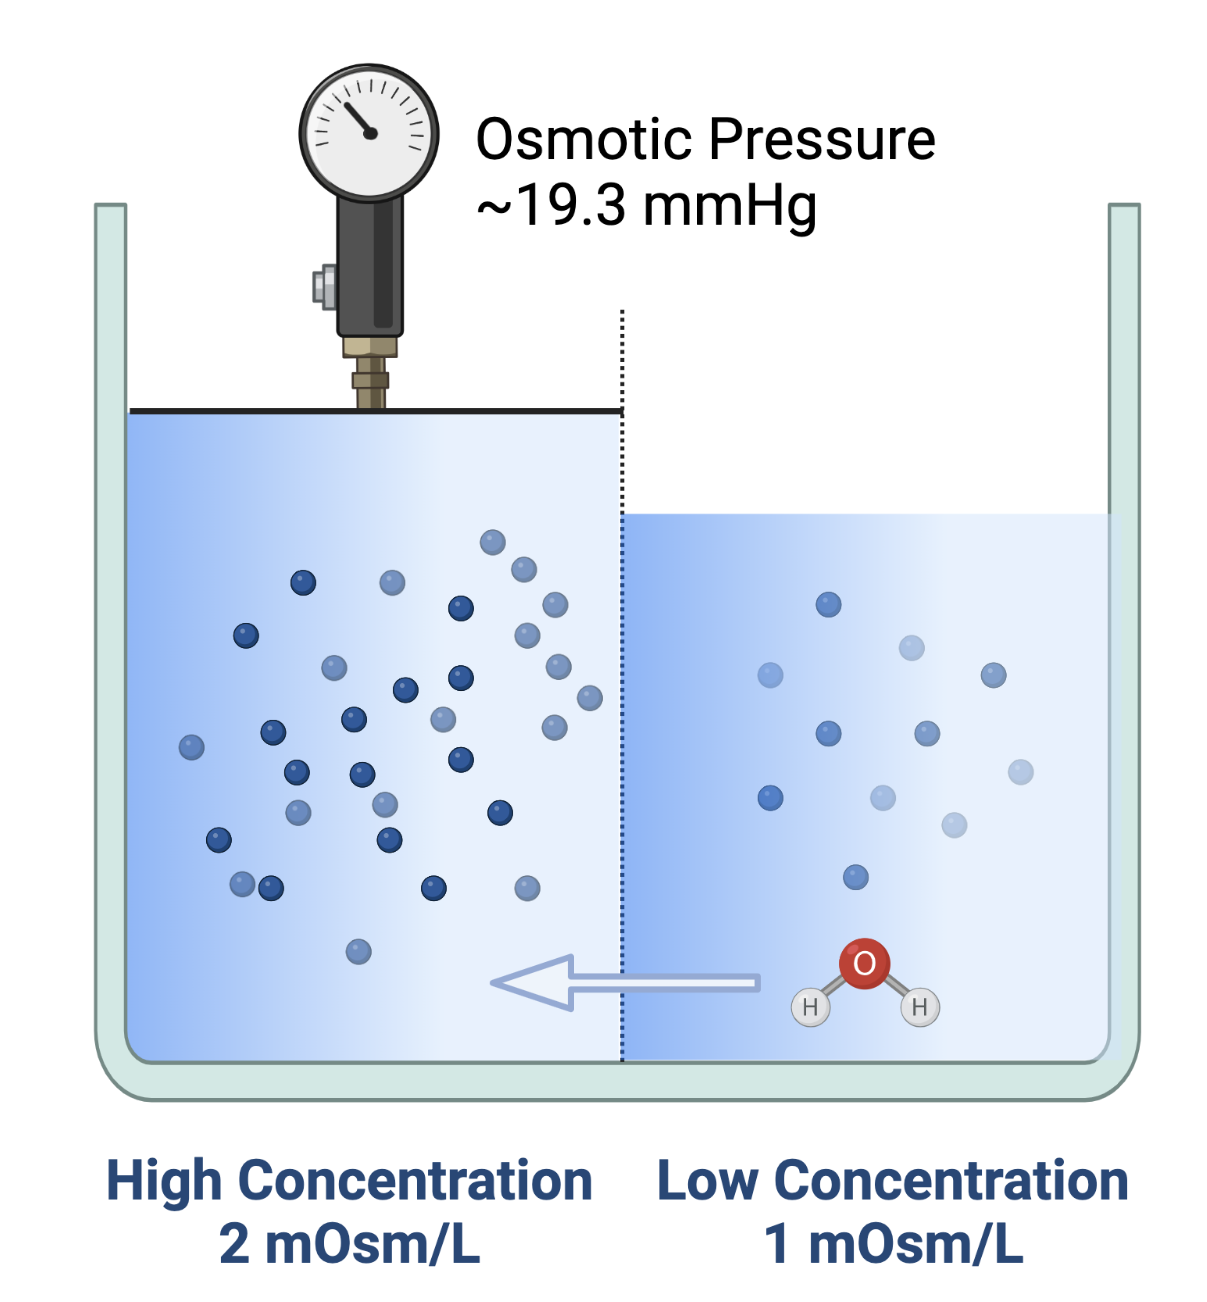
\includegraphics[width=1\linewidth]{./figure/osmotic_pressure.png}
    \caption{Osmotic Pressure \footnotesize{Created with BioRender.com}}
    \label{fig:osmotic_pressure}
\end{figure}

Rapid changes in ICF and ECF can include increases due to large water intake or IV infusions; or decreases (dehydration) associated with sweating, GI fluid loss, excessive urine formation by the kidneys.

Since water moves quickly across the cell membranes the ICF and ECF osmotic pressures quickly equalize. 

Number of osmoles in ECF and ICF remains relatively constant unless solutes are added or lost from the ECF. 

Adding an isotonic solution to ECF- no change in ECF osmolarity, no osmosis, increases ECF volume

Adding hypertonic solution to ECF - ECF osmolarity increases causes osmosis of water out of cells to ECF, increased ECF volume more than already added, decreased ICF volume which increases ICF solute concentration - eventually osmosis of water out of cells stops when osmolarity is equalized

Add hypotonic solution to ECF - ECF osmolarity decreases, causes osmosis of water into cells until osmolarity equalizes both ECF and ICF increase, but ICF to a larger extent



\section{Filtration}


\begin{figure}[!h]
    \centering
    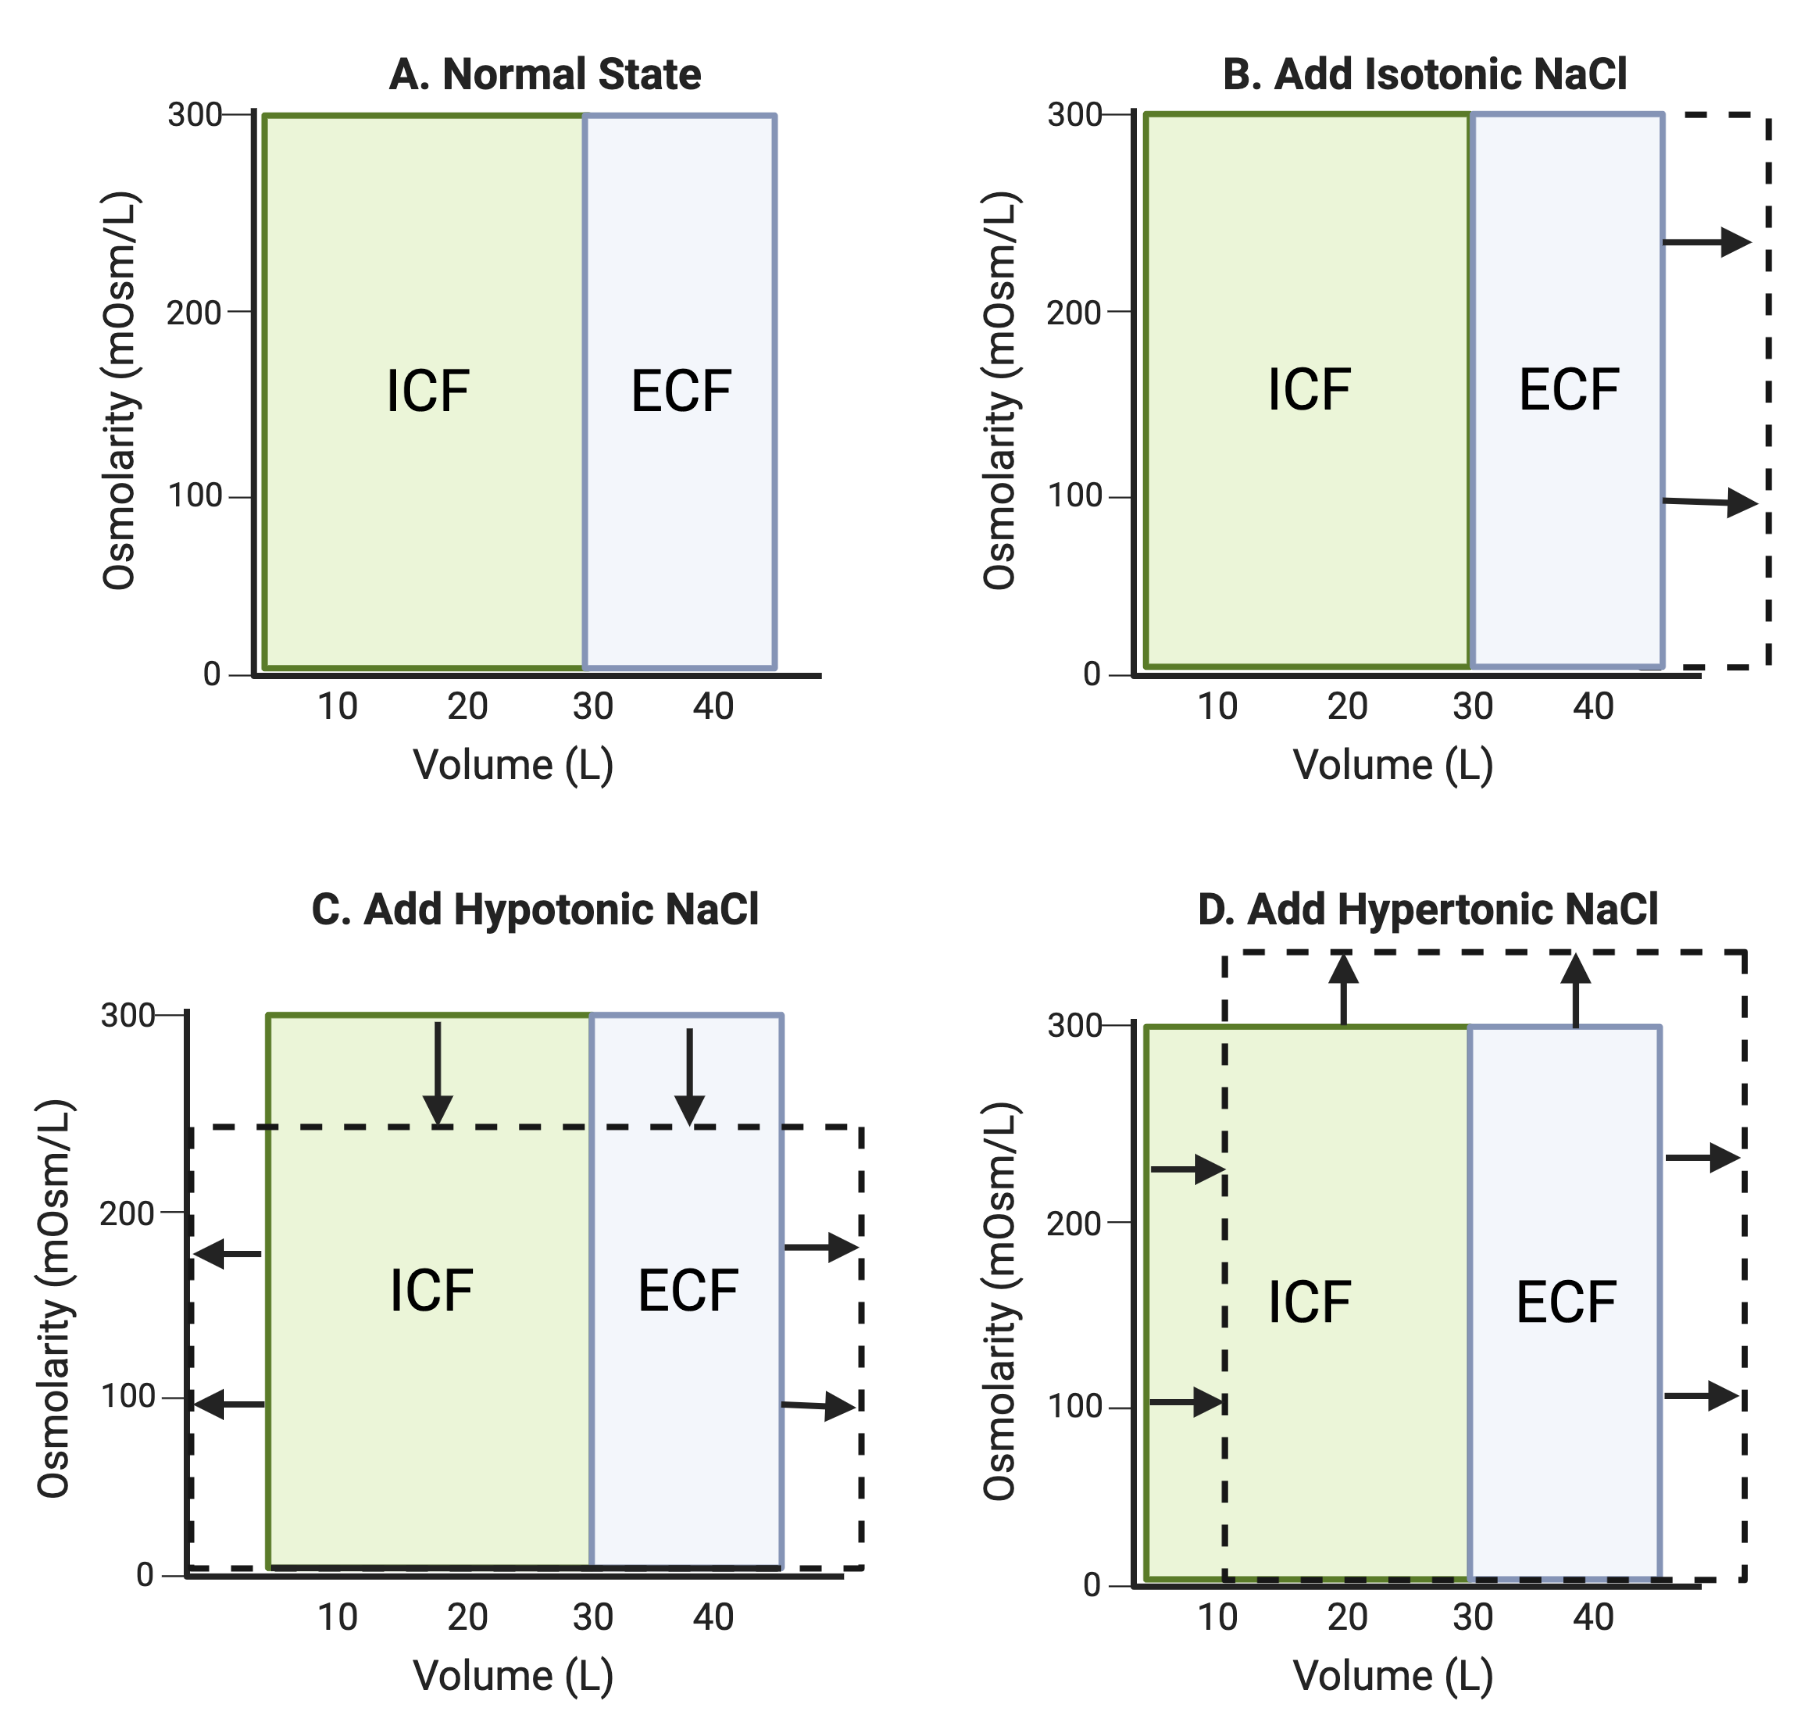
\includegraphics[width=1\linewidth]{./figure/iso_hypo_hypertonic.png}
    \caption{Osmotic Pressure \footnotesize{Created with BioRender.com}}
    \label{fig:iso_hypo_hypertonic}
\end{figure}


\section{Homeostasis}

\subsection{Oxygen \& Carbon Dioxide}

\subsection{Sodium}

\subsection{Potassium}

\subsection{Calcium}

Hypocalcemia, hyperreflexia, muscle cramps, numbness and tingling, twitches
Decreased ECF calcium levels, lowers the threshold potential making it easier to reach threshold for excitation

Hypercalcemia - at high concentrations calcium blocks sodium channels and inhibits depolarization of nerve and muscle fibers, increased calcium raises the threshold for depolarization.[5] This results in diminished deep tendon reflexes (hyporeflexia), and skeletal muscle weakness.

\subsection{Acid Base (pH)}

\subsection{Temperature}

\subsection{Water}



\section{\textit{Clinical Physiology Connections}}

\subsection{Smooth Muscle}

\subsection{Edema}

\subsection{Electrolyte Disturbances}

\subsection{Hyperthermia}

\subsection{Hypotermia}

\printbibliography[heading=subbibintoc]
